\chapter{Karakteristieke groepen en families}\label{ch:g11:functional-groups}

Maak een fles azijn open, een fles nagellakremover, een zak zuurtjes met
peergeur, en loop langs een viskraam: vier geuren, scherp, zoet als een
\omterm{def:g6:solutions-and-solubility:solute}{oplosmiddel}, fruitig en visachtig, en vier verschillende soorten
\omterm{def:g7:atoms-and-molecules:molecule}{moleculen}. Elk \omterm{def:g7:atoms-and-molecules:molecule}{molecuul} dankt zijn geur, en het grootste deel van zijn
chemie, niet aan zijn koolstofskelet maar aan een kleine groep \omterm{def:g7:atoms-and-molecules:atom}{atomen}
die eraan vastzit: zuurstof en waterstof op de ene plek, een
stikstofatoom op de andere. Scheikundigen delen \omterm{def:g11:organic-skeletons:organic}{organische verbindingen}
in naar deze groepen.

\begin{recall}
\omterm{def:g11:organic-skeletons:formulas}{Skeletformules}, de namen van \omterm{def:g11:organic-skeletons:alkane}{alkanen} en \omterm{def:g11:organic-skeletons:alkane}{alkylgroepen}, \omterm{def:g11:organic-skeletons:isomer}{isomeren}
(\cref{ch:g11:organic-skeletons}). \omterm{def:g11:polarity-and-cohesion:polar-bond}{Polaire bindingen} en \omterm{def:g11:polarity-and-cohesion:hydrogen-bond}{waterstofbruggen}
(\cref{ch:g11:polarity-and-cohesion}).
\end{recall}

\begin{omfigure}
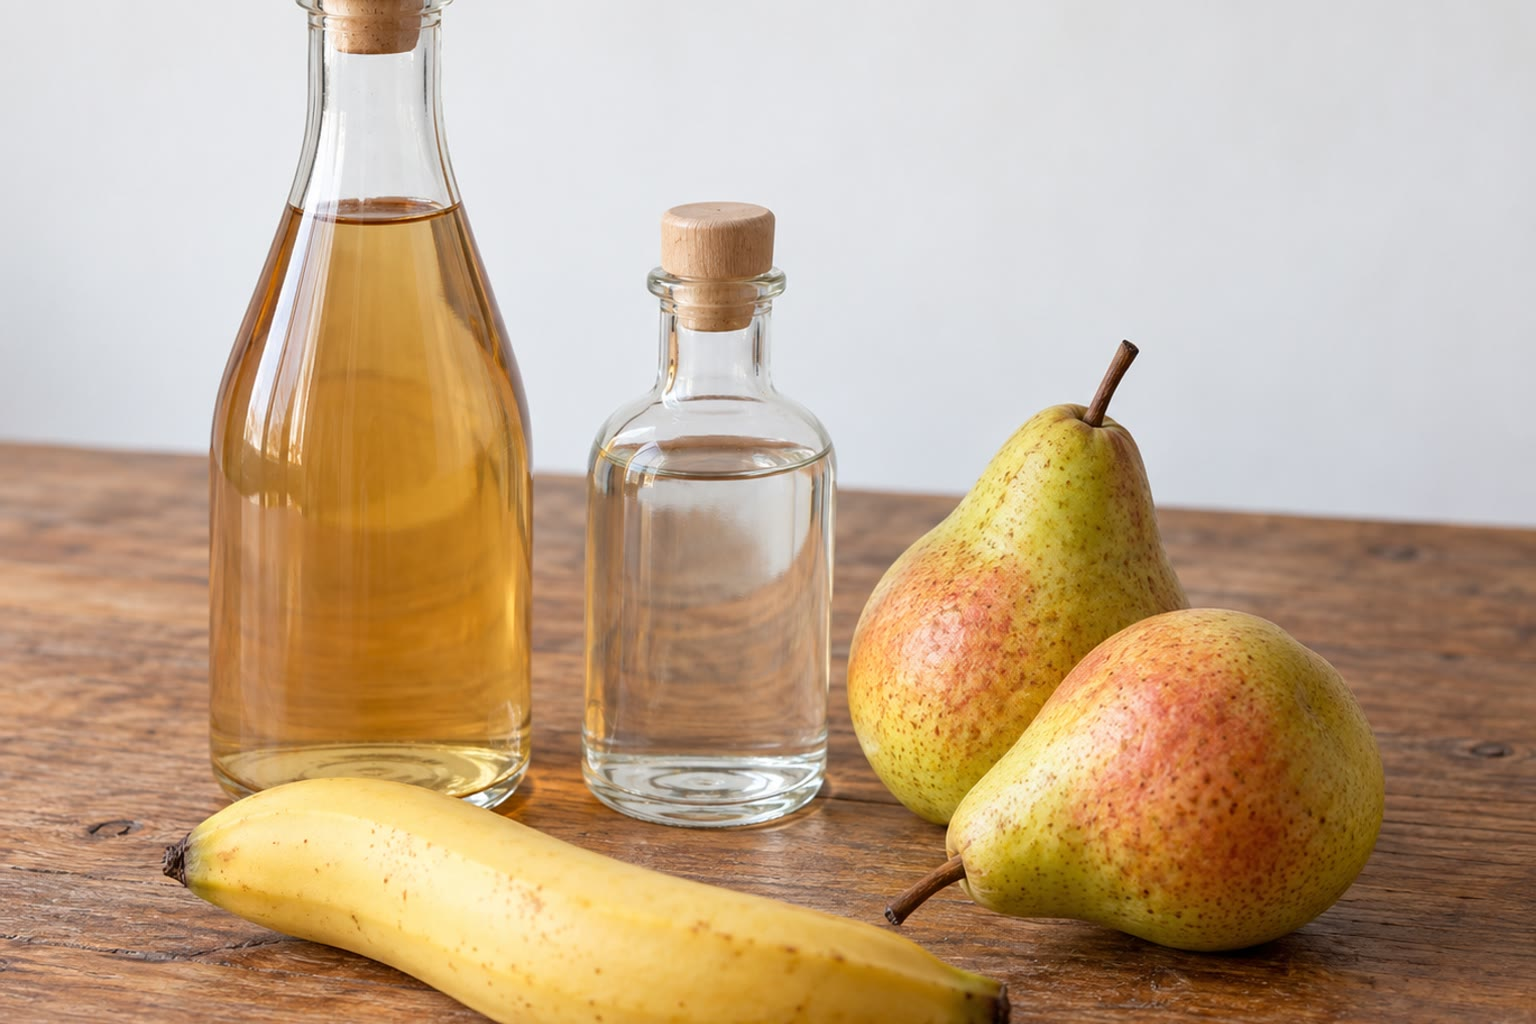
\includegraphics[width=0.5\linewidth]{images/book1/ai/g11-still-life-esters.jpg}

{\small Azijn, een \omterm{def:g6:solutions-and-solubility:solute}{oplosmiddel}, fruit: elke geur komt van een andere
groep \omterm{def:g7:atoms-and-molecules:atom}{atomen} op een koolstofskelet.}
\end{omfigure}

\section{Karakteristieke groepen}

\begin{definition}[Karakteristieke groep]\label{def:g11:functional-groups:functional-group}
Een \emph{karakteristieke groep}\index{karakteristieke groep} is een groep
\omterm{def:g7:atoms-and-molecules:atom}{atomen}, anders dan de koolstof- en waterstofatomen van het skelet die
alleen door enkele bindingen verbonden zijn, die een \omterm{def:g7:atoms-and-molecules:molecule}{molecuul} zijn
kenmerkende reacties geeft. De verbindingen met dezelfde karakteristieke
groep vormen een familie.
\end{definition}

\begin{omfigure}
\renewcommand{\arraystretch}{1.35}
\footnotesize
\begin{tabular}{@{}l@{\enspace}l@{\enspace}l@{\enspace}l@{\enspace}l@{}}
\hline
groep & formule & familie & naamuitgang & voorbeeld \\
\hline
hydroxyl & \ce{-OH} & \omterm{def:g11:functional-groups:alcohol}{alcohol} & \emph{-ol} & ethanol, \ce{CH3-CH2-OH} \\
carbonyl (eind) & \ce{-CHO} & \omterm{def:g11:functional-groups:carbonyl}{aldehyde} & \emph{-al} & ethanal, \ce{CH3-CHO} \\
carbonyl (midden) & \ce{C-CO-C} & \omterm{def:g11:functional-groups:carbonyl}{keton} & \emph{-on} & propanon, \ce{CH3-CO-CH3} \\
carboxyl & \ce{-COOH} & \omterm{def:g11:functional-groups:carboxylic-acid}{carbonzuur} & \emph{-zuur} & ethaanzuur, \ce{CH3-COOH} \\
\omterm{def:g11:functional-groups:carboxylic-acid}{ester} & \ce{C-COO-C} & \omterm{def:g11:functional-groups:carboxylic-acid}{ester} & \emph{-yl \ldots-oaat} & ethylethanoaat, \ce{CH3-COO-CH2-CH3} \\
\omterm{def:g11:functional-groups:amine}{amine} & \ce{-NH2} & \omterm{def:g11:functional-groups:amine}{amine} & \emph{-amine} & ethaanamine, \ce{CH3-CH2-NH2} \\
\omterm{def:g11:functional-groups:amine}{amide} & \ce{-CONH2} & \omterm{def:g11:functional-groups:amine}{amide} & \emph{-amide} & ethaanamide, \ce{CH3-CONH2} \\
\omterm{def:g10:electron-shells:family}{halogeen} & \ce{C-X} & \omterm{def:g11:functional-groups:halogenoalkane}{halogeenalkaan} & voorvoegsel \emph{chloor-}, \ldots & chloormethaan, \ce{CH3Cl} \\
\omterm{def:g10:lewis-and-shape:multiple-bond}{dubbele binding} & \ce{C=C} & \omterm{def:g11:functional-groups:halogenoalkane}{alkeen} & \emph{-een} & etheen, \ce{CH2=CH2} \\
\hline
\end{tabular}\par\medskip

\setchemfig{atom sep=1.4em}
\begin{tabular}{@{}c@{\quad}c@{\quad}c@{\quad}c@{\quad}c@{}}
\chemfig{R-C(=[2]O)-H} & \chemfig{R-C(=[2]O)-R'} & \chemfig{R-C(=[2]O)-O-H} &
\chemfig{R-C(=[2]O)-O-R'} & \chemfig{R-C(=[2]O)-N(-[1]H)-[7]H} \\
\small \omterm{def:g11:functional-groups:carbonyl}{aldehyde} & \small \omterm{def:g11:functional-groups:carbonyl}{keton} & \small \omterm{def:g11:functional-groups:carboxylic-acid}{carbonzuur} & \small \omterm{def:g11:functional-groups:carboxylic-acid}{ester} &
\small \omterm{def:g11:functional-groups:amine}{amide}
\end{tabular}\par\medskip

{\small De belangrijkste \omterm{def:g11:functional-groups:functional-group}{karakteristieke groepen}, en de vijf die op een
carbonylgroep \ce{C=O} gebouwd zijn, volledig getekend. R en R$'$ staan
voor koolstofketens (\omterm{def:g11:organic-skeletons:alkane}{alkylgroepen}) en X voor een halogeenatoom (F, Cl,
Br, I).}
\end{omfigure}

\section{Alcoholen en hun klasse}

\begin{definition}[Alcohol, klasse van een alcohol]\label{def:g11:functional-groups:alcohol}
Een \emph{alcohol}\index{alcohol} heeft een hydroxylgroep \ce{-OH}
gebonden aan een koolstofatoom dat alleen enkele bindingen heeft. De
\emph{klasse van een alcohol}\index{klasse van een alcohol} is primair,
secundair of tertiair, naargelang het koolstofatoom met de \ce{-OH}
gebonden is aan één, twee of drie andere koolstofatomen. (Methanol,
\ce{CH3OH}, waarvan het koolstofatoom aan geen enkel ander gebonden is,
wordt bij de primaire alcoholen gerekend.)
\end{definition}

\begin{omfigure}
\setchemfig{atom sep=1.9em}
\begin{tabular}{ccc}
\chemfig{-[:30]-[:-30]-[:30]-[:-30]OH} &
\chemfig{-[:30](-[:90]OH)-[:-30]-[:30]} &
\chemfig{-[:0](-[:90]OH)(-[:-90])-[:0]} \\[4pt]
\small butaan-1-ol & \small butaan-2-ol & \small 2-methylpropaan-2-ol \\
\small \textbf{primair} & \small \textbf{secundair} & \small \textbf{tertiair} \\
\small (C van \ce{-OH}: 1 koolstofbuur) & \small (2 buren) &
\small (3 buren)
\end{tabular}

{\small Drie \omterm{def:g11:organic-skeletons:isomer}{isomeren} \ce{C4H10O}, drie klassen van \omterm{def:g11:functional-groups:alcohol}{alcoholen}.}
\end{omfigure}

\section{Aldehyden, ketonen, zuren en esters}

\begin{definition}[Aldehyde, keton]\label{def:g11:functional-groups:carbonyl}
Een carbonylgroep is een \omterm{def:g10:lewis-and-shape:multiple-bond}{dubbele binding} \ce{C=O}. Zit het koolstofatoom
ervan aan het uiteinde van de keten (gebonden aan minstens één
waterstofatoom), dan is de verbinding een
\emph{aldehyde}\index{aldehyde}; zit het midden in de keten (gebonden aan
twee koolstofatomen), dan is de verbinding een \emph{keton}\index{keton}.
\end{definition}

\begin{definition}[Carbonzuur, ester]\label{def:g11:functional-groups:carboxylic-acid}
Een \emph{carbonzuur}\index{carbonzuur} heeft een carboxylgroep
\ce{-COOH}, een carbonyl- en een hydroxylgroep op hetzelfde
koolstofatoom. Een \emph{ester}\index{ester} heeft de groep \ce{-COO-}
tussen twee koolstofketens: hij is verwant aan een zuur waarvan de
\ce{-OH} vervangen is door een \ce{-O-}R$'$ die van een \omterm{def:g11:functional-groups:alcohol}{alcohol} komt.
\end{definition}

\begin{example}[Ethylethanoaat]\label{ex:g11:functional-groups:ethyl-ethanoate}
Het \omterm{def:g6:solutions-and-solubility:solute}{oplosmiddel} ethylethanoaat, \ce{CH3-COO-CH2-CH3}, ruikt naar
peerzuurtjes en nagellakremover. Het ``zuurdeel'', \ce{CH3-CO}, komt van
ethaanzuur \ce{CH3-COOH} en geeft het tweede deel van de naam,
\emph{ethanoaat}; het ``alcoholdeel'', \ce{O-CH2-CH3}, komt van ethanol
\ce{CH3-CH2-OH} en geeft het eerste deel, \emph{ethyl}. Een later
hoofdstuk laat zien hoe je een \omterm{def:g11:functional-groups:carboxylic-acid}{ester} maakt uit zijn zuur en zijn \omterm{def:g11:functional-groups:alcohol}{alcohol}.
\end{example}

\begin{omfigure}
\setchemfig{atom sep=2.2em}
\chemfig{@{a}H_3C-@{c}C(=[2]@{o}O)-@{x}O-CH_2-@{z}CH_3}
\chemmove{
  \fill[omProp, opacity=0.14, rounded corners]
    ($(a.south west)+(-0.12,-0.15)$) rectangle ($(o.north east)+(0.25,0.12)$);
  \fill[omDef, opacity=0.14, rounded corners]
    ($(x.south west)+(-0.2,-0.15)$) rectangle ($(z.north east)+(0.4,0.75)$);
  \node[omProp, anchor=north east, align=right, font=\small] at ($(c.south)+(0.15,-0.25)$)
    {zuurdeel, van ethaanzuur:\\ \emph{ethanoaat}};
  \node[omDef, anchor=north west, align=left, font=\small] at ($(x.south)+(0.05,-0.25)$)
    {alcoholdeel, van ethanol:\\ \emph{ethyl}};}
\par\vspace{1.4cm}

{\small De naam van een \omterm{def:g11:functional-groups:carboxylic-acid}{ester}: het alcoholdeel geeft een alkylnaam
(\emph{ethyl}), het zuurdeel een uitgang op \emph{-oaat}
(\emph{ethanoaat}); de naam is ``ethylethanoaat''.}
\end{omfigure}

\section{Aminen, amiden, halogeenalkanen en alkenen}


\begin{definition}[Amine, amide]\label{def:g11:functional-groups:amine}
Een \emph{amine}\index{amine} heeft een stikstofatoom dat met een enkele
binding aan een koolstofketen gebonden is, zoals in \ce{-NH2}. Een
\emph{amide}\index{amide} heeft een stikstofatoom dat gebonden is aan het
koolstofatoom van een carbonylgroep, zoals in \ce{-CO-NH2}.
\end{definition}

\begin{definition}[Halogeenalkaan, alkeen]\label{def:g11:functional-groups:halogenoalkane}
Een \emph{halogeenalkaan}\index{halogeenalkaan} is een \omterm{def:g11:organic-skeletons:alkane}{alkaan} waarin een
of meer waterstofatomen vervangen zijn door halogeenatomen (F, Cl, Br,
I). Een \emph{alkeen}\index{alkeen} heeft een \omterm{def:g10:lewis-and-shape:multiple-bond}{dubbele binding} tussen twee
koolstofatomen, \ce{C=C}.
\end{definition}

\begin{remark}[Geuren en groepen]\label{rem:g11:functional-groups:smells}
Veel kleine \omterm{def:g11:functional-groups:amine}{aminen} ruiken naar rotte vis, en de geur van vis die niet
meer vers is, komt grotendeels van hen. Veel kleine \omterm{def:g11:functional-groups:carboxylic-acid}{esters} ruiken naar
fruit. Kleine \omterm{def:g11:functional-groups:carboxylic-acid}{carbonzuren} ruiken scherp, zoals azijn; propanon, een
\omterm{def:g11:functional-groups:carbonyl}{keton}, is de bekende oplosmiddelgeur van nagellakremover.
\end{remark}

\section{Naamgeving}

\begin{method}[Een organische verbinding met één karakteristieke groep een naam geven]\label{met:g11:functional-groups:naming}
\begin{enumerate}
  \item Zoek de langste koolstofketen die het koolstofatoom van de
        \omterm{def:g11:functional-groups:functional-group}{karakteristieke groep} \emph{bevat} (of, bij een \omterm{def:g11:functional-groups:alcohol}{alcohol} of een
        \omterm{def:g11:functional-groups:amine}{amine}, het koolstofatoom dat de groep draagt): die geeft de stam.
  \item Nummer de keten vanaf het uiteinde dat de \omterm{def:g11:functional-groups:functional-group}{karakteristieke groep}
        het laagste nummer geeft.
  \item Laat de alkaannaam volgen door de uitgang van de familie, zo
        nodig met de plaats van de groep ervoor: propaan-2-ol,
        butaan-2-on; zonder nummer valt de \emph{a} van \mbox{-aan} weg
        voor een klinker (propanal, propanon). (\omterm{def:g11:functional-groups:carbonyl}{Aldehyden}, zuren en
        \omterm{def:g11:functional-groups:amine}{amiden} hebben hun groep op koolstofatoom 1: geen nummer.)
  \item Voeg de alkylsubstituenten met hun plaats toe als voorvoegsels,
        zoals bij \omterm{def:g11:organic-skeletons:alkane}{alkanen}; een \omterm{def:g10:electron-shells:family}{halogeen} is altijd een voorvoegsel
        (2-chloorpropaan).
\end{enumerate}
\end{method}

\begin{example}[Vier namen]\label{ex:g11:functional-groups:names}
\setchemfig{atom sep=1.7em}
\chemfig{-[:30](-[:90]OH)-[:-30]} is propaan-2-ol (een secundaire
\omterm{def:g11:functional-groups:alcohol}{alcohol});
\chemfig{-[:30](=[:90]O)-[:-30]-[:30]} is butaan-2-on;
\chemfig{-[:30]-[:-30]-[:30](=[:90]O)-[:-30]OH} is butaanzuur;
\chemfig{-[:30](-[:90])-[:-30]-[:30]=[:-30]O} is 3-methylbutanal.
\end{example}

\begin{omfigure}
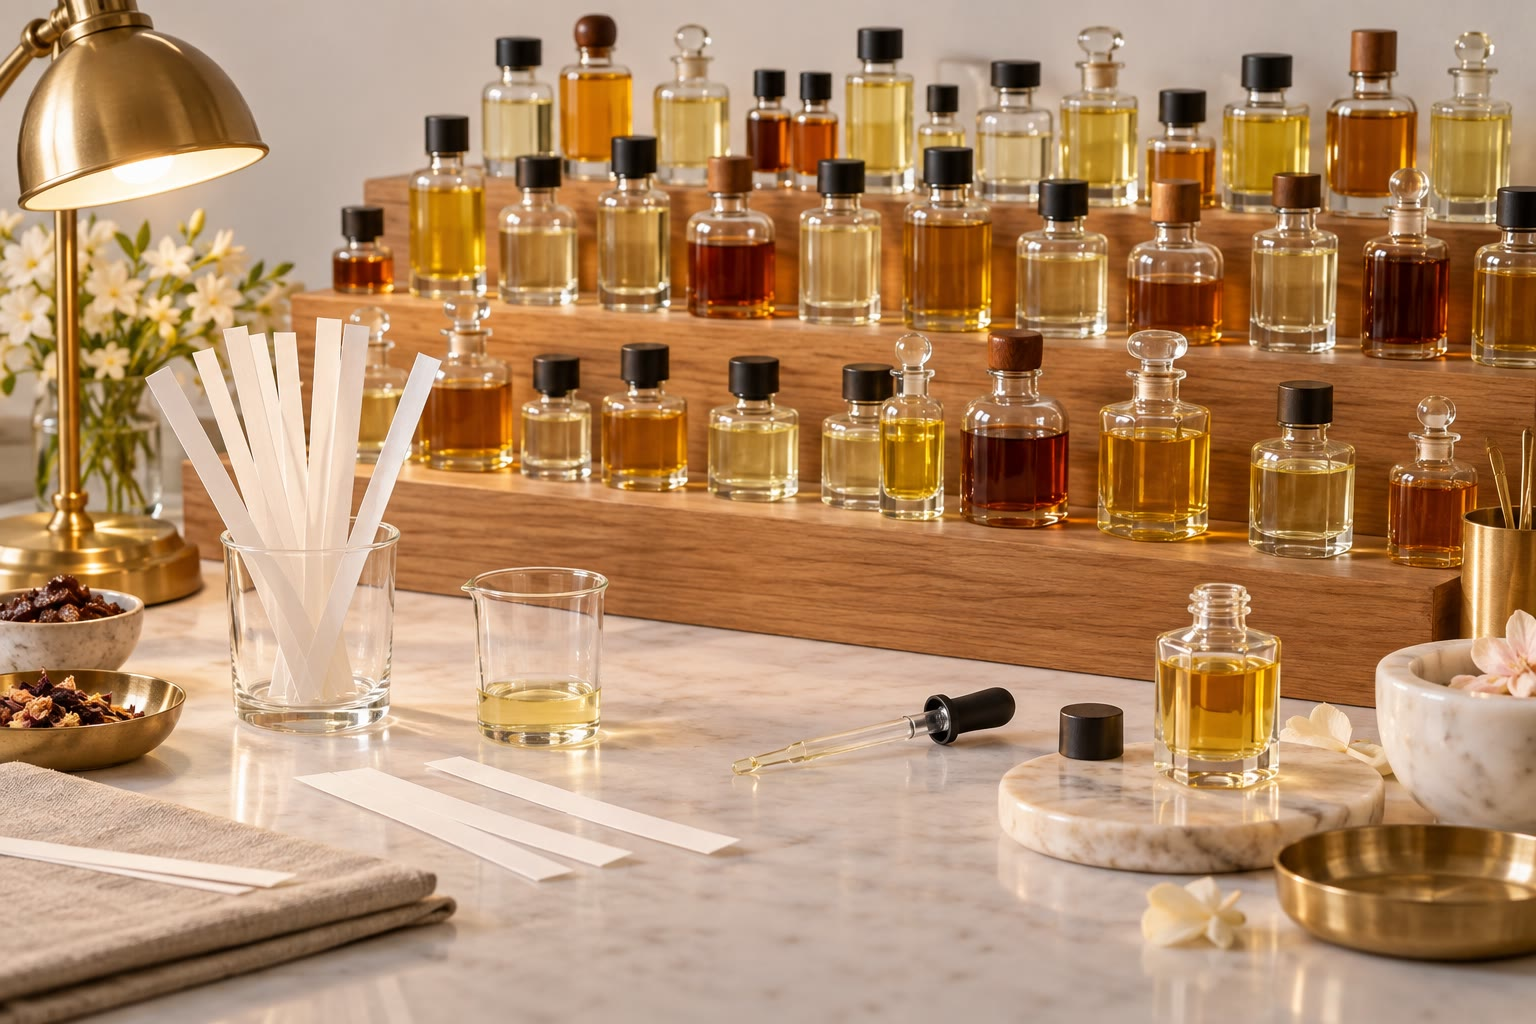
\includegraphics[width=0.48\linewidth]{images/book1/ai/g11-perfumer-lab.jpg}

{\small De werktafel van een parfumeur: veel van de flesjes bevatten
\omterm{def:g11:functional-groups:carboxylic-acid}{esters}, \omterm{def:g11:functional-groups:alcohol}{alcoholen}, \omterm{def:g11:functional-groups:carbonyl}{aldehyden} en \omterm{def:g11:functional-groups:carbonyl}{ketonen}.}
\end{omfigure}

\begin{safety}{\ghs[0.82cm]{GHS02}\ghs[0.82cm]{GHS05}\ghs[0.82cm]{GHS07}}
% ledger: ghs:acetone, ghs:acetic-acid
Propanon is licht ontvlambaar en irriterend voor de ogen; de damp maakt
slaperig. Zuiver ethaanzuur is ontvlambaar en veroorzaakt ernstige
brandwonden aan huid en ogen; azijn is een verdunde oplossing ervan. Een
geur test je nooit door aan een kolf te snuiven: je waaiert de damp
voorzichtig met je hand naar je neus toe, en alleen als de docent dat
zegt.
\end{safety}

\section{Oefeningen}


\begin{exercise}[$\star$]\label{exo:g11:functional-groups:1}
Noem de \omterm{def:g11:functional-groups:functional-group}{karakteristieke groep} en de familie van elke verbinding:
\ce{CH3-CH2-CH2-OH}; \ce{CH3-CO-CH2-CH3}; \ce{CH3-CH2-COOH};
\ce{CH3-COO-CH3}; \ce{CH3-CH2-NH2}.
\end{exercise}

\begin{exercise}[$\star$]\label{exo:g11:functional-groups:2}
Geef de naam van: \ce{CH3-OH}; \ce{CH3-CH2-CH2-OH}; \ce{HCOOH};
\ce{CH3-CH2-CHO}; \ce{CH3-CO-CH3}.
\end{exercise}

\begin{exercise}[$\star$]\label{exo:g11:functional-groups:3}
Tot welke familie hoort elke verbinding: butaan-2-ol, pentanal,
methylpropanoaat, propaanamide, 2-broompropaan, but-1-een?
\end{exercise}

\begin{exercise}[$\star$]\label{exo:g11:functional-groups:4}
Schrijf de \omterm{def:g11:organic-skeletons:formulas}{beknopte structuurformules} op van propanal en van propanon.
Welke is het \omterm{def:g11:functional-groups:carbonyl}{aldehyde}? Hoe zie je dat?
\end{exercise}

\begin{exercise}[$\star$]\label{exo:g11:functional-groups:5}
Geef de klasse van propaan-1-ol, propaan-2-ol en 2-methylpropaan-2-ol.
\end{exercise}

\begin{exercise}[$\star\star$]\label{exo:g11:functional-groups:6}
Teken de \omterm{def:g11:organic-skeletons:formulas}{skeletformules} van pentaan-3-ol, 2-methylbutaanzuur,
hexaan-2-on en propylethanoaat.
\end{exercise}

\begin{exercise}[$\star\star$]\label{exo:g11:functional-groups:7}
Propanal en propanon hebben dezelfde \omterm{def:g11:organic-skeletons:formulas}{molecuulformule}. Geef die. Zijn het
\omterm{def:g11:organic-skeletons:isomer}{isomeren}? Hebben ze dezelfde \omterm{def:g11:functional-groups:functional-group}{karakteristieke groep}?
\end{exercise}

\begin{exercise}[$\star\star$]\label{exo:g11:functional-groups:8}
Schrijf de \omterm{def:g11:organic-skeletons:formulas}{beknopte structuurformule} en de naam op van de \omterm{def:g11:functional-groups:carboxylic-acid}{ester} waarvan
het zuurdeel van methaanzuur \ce{HCOOH} komt en het alcoholdeel van
ethanol; daarna van de \omterm{def:g11:functional-groups:carboxylic-acid}{ester} uit ethaanzuur en propaan-1-ol.
\end{exercise}

\begin{exercise}[$\star\star$]\label{exo:g11:functional-groups:9}
Geef de namen van de \omterm{def:g11:functional-groups:carboxylic-acid}{esters} \ce{CH3-COO-CH3}, \ce{CH3-CH2-COO-CH2-CH3} en
\ce{HCOO-CH3}, en noem het zuur en de \omterm{def:g11:functional-groups:alcohol}{alcohol} waaraan elk verwant is.
\end{exercise}

\begin{exercise}[$\star\star$]\label{exo:g11:functional-groups:10}
Teken de vier \omterm{def:g11:functional-groups:alcohol}{alcoholen} met formule \ce{C4H10O}, geef hun namen, en geef
van elk de klasse.
\end{exercise}

\begin{exercise}[$\star\star$]\label{exo:g11:functional-groups:11}
Met de tabel van groepen: wat is de familie van \ce{CH3-CO-NH2}? Welke
uitgang krijgt de naam van een \omterm{def:g11:functional-groups:halogenoalkane}{alkeen}? Welke families hebben een
carbonylgroep met een zuurstof- of stikstofatoom op hetzelfde
koolstofatoom?
\end{exercise}

\begin{exercise}[$\star\star\star$]\label{exo:g11:functional-groups:12}
Omcirkel en benoem de \omterm{def:g11:functional-groups:functional-group}{karakteristieke groepen} van aspirine en van
paracetamol. (Een \ce{-OH} die direct aan een ring zoals die van
paracetamol gebonden is, heet een fenolgroep; die gedraagt zich anders
dan een \omterm{def:g11:functional-groups:alcohol}{alcohol}.)
\begin{center}
\setchemfig{atom sep=1.6em}
\chemfig{*6(-=-(-COOH)=(-O-[:150]C(=[:90]O)-[:210]H_3C)-=)}
\qquad
\chemfig{*6((-OH)=-=(-N(-[2]H)-[7]C(=[6]O)-[1]CH_3)-=-)}
\\[2pt] \small aspirine \hspace{4.2cm} paracetamol
\end{center}
\end{exercise}

\begin{exercise}[$\star\star\star$]\label{exo:g11:functional-groups:13}
% ledger: bp:C2H5OH, bp:CH3OCH3
Ethanol \ce{CH3-CH2-OH} en methoxymethaan \ce{CH3-O-CH3} hebben dezelfde
\omterm{def:g11:organic-skeletons:formulas}{molecuulformule}. Geef die. Methoxymethaan hoort bij een familie die niet
in de tabel staat, de ethers. Welke van de twee kan \omterm{def:g11:polarity-and-cohesion:hydrogen-bond}{waterstofbruggen}
vormen tussen zijn eigen \omterm{def:g7:atoms-and-molecules:molecule}{moleculen}? Welke kookt hoger (de ene kookt bij
\qty{78}{\celsius}, de andere bij \qty{-25}{\celsius})?
\end{exercise}

\begin{exercise}[$\star\star\star$]\label{exo:g11:functional-groups:14}
Melkzuur, dat vermoeide spieren maken, is
\chemfig{CH_3-CH(-[2]OH)-COOH}. Noem de twee \omterm{def:g11:functional-groups:functional-group}{karakteristieke groepen}. Als
een \omterm{def:g7:atoms-and-molecules:molecule}{molecuul} een zuurgroep en nog een andere groep heeft, geeft het zuur
de uitgang en wordt de andere groep een voorvoegsel (\emph{hydroxy-} voor
\ce{-OH}, \emph{amino-} voor \ce{-NH2}). Geef de naam van melkzuur, en
daarna van glycine, \ce{H2N-CH2-COOH}.
\end{exercise}

\begin{exercise}[$\star\star\star$]\label{exo:g11:functional-groups:15}
Wijn die open aan de \omterm{def:g4:air-a-mixture-of-gases:air}{lucht} staat, wordt azijn: ethanol wordt via ethanal
ethaanzuur. Schrijf de \omterm{def:g11:organic-skeletons:formulas}{beknopte structuurformules} en de \omterm{def:g11:organic-skeletons:formulas}{molecuulformules}
van de drie verbindingen op, en hun families. Wat verandert er bij elke
stap in de formule?
\end{exercise}

\section{Probleem: Fruitaroma's}

\begin{problem}[{Weekendprobleem --- een aromachemicus bouwt de geur van
banaan na: wat is de molaire massa van het sleutelmolecuul?}]
\label{pb:g11:functional-groups:1}
% ledger: aw:C, aw:H, aw:O
Een aromachemicus heeft vijf verbindingen op haar werktafel:
\begin{center}
\begin{tabular}{ll}
A & \chemfig{CH_3-C(=[2]O)-O-CH_2-CH_2-CH(-[2]CH_3)-CH_3} \\[16pt]
B & \chemfig{HO-CH_2-CH_2-CH(-[2]CH_3)-CH_3} \\[10pt]
C & \ce{CH3-COOH} \\
D & \ce{CH3-CH2-CH2-CH2-CH2-CHO} \\
E & \ce{CH3-CH2-CH2-COO-CH2-CH3}
\end{tabular}
\end{center}
A ruikt naar banaan en peerzuurtjes, B naar mout, C naar azijn, D naar
gemaaid gras, E naar ananas.

\medskip
\noindent\textbf{Deel I --- Groepen en families.}
\begin{enumerate}
  \item Noem de \omterm{def:g11:functional-groups:functional-group}{karakteristieke groep} van elke verbinding.
  \item Geef de familie van elke verbinding.
  \item Welke verbindingen zijn \omterm{def:g11:functional-groups:carboxylic-acid}{esters}? Welke geuren hebben ze?
  \item Wat is de klasse van de \omterm{def:g11:functional-groups:alcohol}{alcohol} B?
  \item Geef de \omterm{def:g11:organic-skeletons:formulas}{molecuulformule} van D, en teken een \omterm{def:g11:organic-skeletons:isomer}{isomeer} van D dat een
        \omterm{def:g11:functional-groups:carbonyl}{keton} is.
\end{enumerate}

\medskip
\noindent\textbf{Deel II --- Namen.}
\begin{enumerate}[resume]
  \item Geef de naam van B (zoek de langste keten die het koolstofatoom
        met de \ce{-OH} bevat).
  \item Geef de namen van C en D.
  \item Geef de naam van E, en noem het zuur en de \omterm{def:g11:functional-groups:alcohol}{alcohol} waaraan het
        verwant is.
  \item Verklaar de naam van A, 3-methylbutylethanoaat: welk deel komt van
        het zuur, welk van de \omterm{def:g11:functional-groups:alcohol}{alcohol}?
\end{enumerate}

\medskip
\noindent\textbf{Deel III --- Uit een zuur en een \omterm{def:g11:functional-groups:alcohol}{alcohol}.}
\begin{enumerate}[resume]
  \item Aan welke twee verbindingen van de werktafel is A verwant?
  \item Geef de \omterm{def:g11:organic-skeletons:formulas}{molecuulformules} van A, B en C.
  \item Een \omterm{def:g11:functional-groups:carboxylic-acid}{ester} ontstaat uit zijn zuur en zijn \omterm{def:g11:functional-groups:alcohol}{alcohol}, waarbij één
        klein \omterm{def:g7:atoms-and-molecules:molecule}{molecuul} vrijkomt. Bepaal met de formules welk.
  \item Schrijf de vergelijking van de vorming van A op, in
        \omterm{def:g11:organic-skeletons:formulas}{molecuulformules}, en controleer dat ze klopt.
\end{enumerate}

\medskip
\noindent\textbf{Deel IV --- \omterm{def:g10:the-mole:molar-mass}{Molaire massa's}.}
\begin{enumerate}[resume]
  \item Bereken de \omterm{def:g10:the-mole:molar-mass}{molaire massa's} van B en C.
  \item Leid de \omterm{def:g10:the-mole:molar-mass}{molaire massa} van A af uit de vergelijking van vraag 13.
  \item Bereken de \omterm{def:g10:the-mole:molar-mass}{molaire massa} van A rechtstreeks uit zijn formule, en
        vergelijk.
  \item Van een onbekend fruitig monster wordt een \omterm{def:g10:the-mole:molar-mass}{molaire massa} van
        ongeveer \qty{116}{g/mol} gevonden. Is het A of E?
  \item Heptaanzuur, \ce{CH3-(CH2)5-COOH}, ruikt ranzig. Laat zien dat het
        een \omterm{def:g11:organic-skeletons:isomer}{isomeer} van A is. Kan een \omterm{def:g10:the-mole:molar-mass}{molaire massa} alleen een verbinding
        identificeren?
  \item Waarom zeggen scheikundigen dat de geur evenzeer bij de
        \omterm{def:g11:functional-groups:functional-group}{karakteristieke groep} hoort als bij het skelet? Gebruik A en
        heptaanzuur.
  \item Geef het eindantwoord: wat is de \omterm{def:g10:the-mole:molar-mass}{molaire massa} van de bananenester,
        3-methylbutylethanoaat?
\end{enumerate}
\end{problem}
